\documentclass[11pt,letterpaper]{article}
\usepackage[lmargin=1in,rmargin=1in,tmargin=1in,bmargin=1in]{geometry}
\usepackage{../style/homework}
\usepackage{../style/commands}
\setbool{quotetype}{false} % True: Side; False: Under
\setbool{hideans}{false} % Student: True; Instructor: False

% -------------------
% Content
% -------------------
\begin{document}

\homework{1: Due 05/24}{It is easy to forget now, how effervescent and free we all felt that summer.}{Anna Godbersen}

% Problem 1
\problem{10} Showing all your work and simplifying as much as possible, compute each of the following:
        \begin{enumerate}[(a)]
        \item $15/5(1 + 2)$
        \item $20/(4(2 + 3))$
        \item $\dfrac{4^2/2 - 8 + 3 \cdot -2}{(12 - 4)(4 - 5)}$
        \item $\dfrac{8 - 12}{-2^2} + 7 \cdot 12/2$
        \item $4(-1)^3 - 2(-1)^3 + 6 \cdot 5/4$
        \end{enumerate} \pspace

\sol 
\begin{enumerate}[(a)]
\item 
	\[
	15/5(1 + 2)= 15/5(3)= 3(3)= 9
	\] \pspace

\item 
	\[
	20/(4(2 + 3))= 20/(4(5))= 20/20= 1
	\] \pspace

\item 
	\[
	\dfrac{4^2/2 - 8 + 3 \cdot -2}{(12 - 4)(4 - 5)}= \dfrac{4^2/2 - 8 + 3 \cdot -2}{8 \cdot -1}= \dfrac{16/2 - 8 - 6}{-8}= \dfrac{8 - 8 - 6}{-8}= \dfrac{-6}{-8}= \dfrac{6}{8}= \dfrac{3}{4}
	\] \pspace

\item 
	\[
	\dfrac{8 - 12}{-2^2} + 7 \cdot 12/2= \dfrac{-4}{-4} + 7 \cdot 6= 1 + 42= 43
	\] \pspace

\item 
	\[
	4(-1)^3 - 2(-1)^3 + 6 \cdot 5/4= 4(-1) - 2(-1) + 30/4= -4 + 2 + \dfrac{15}{2}= -2 + \dfrac{15}{2}= \dfrac{-4}{2} + \dfrac{15}{2}= \dfrac{11}{2}
	\]
\end{enumerate}



\newpage



% Problem 2
\problem{10} Showing all your work, find the prime factorizations of the following integers:
        \begin{enumerate}[(a)]
        \item $90$
        \item $141$
        \item $149$
        \item $27$
        \item $185$
        \end{enumerate} \pspace

\sol
\begin{enumerate}[(a)]
\item $90= 2 \cdot 3^2 \cdot 5$
	\[
	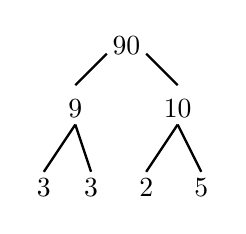
\begin{tikzpicture}
	\node at (-0.15,0) {$90$};
	\draw[line width=0.03cm] (-0.4,-0.1) -- (-0.8,-0.5);
	\node at (-0.8,-0.8) {$9$};
	\draw[line width=0.03cm]  (0.1,-0.1) -- (0.5,-0.5);
	\node at (0.5,-0.8) {$10$};
		
	\draw[line width=0.03cm] (-0.8,-1) -- (-1.2,-1.6);
	\node at (-1.2,-1.8) {$3$};
	\draw[line width=0.03cm] (-0.8,-1) -- (-0.6,-1.6);
	\node at (-0.6,-1.8) {$3$};
	
	\draw[line width=0.03cm] (0.5,-1) -- (0.1,-1.6);
	\node at (0.1,-1.8) {$2$};
	\draw[line width=0.03cm] (0.5,-1) -- (0.8,-1.6);
	\node at (0.8,-1.8) {$5$};
	\end{tikzpicture}
	\] \pspace

\item $141= 3 \cdot 47$
	\[
	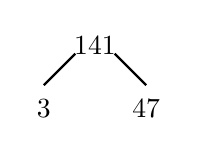
\begin{tikzpicture}
	\node at (-0.15,0) {$141$};
	\draw[line width=0.03cm] (-0.4,-0.1) -- (-0.8,-0.5);
	\node at (-0.8,-0.8) {$3$};
	\draw[line width=0.03cm]  (0.1,-0.1) -- (0.5,-0.5);
	\node at (0.5,-0.8) {$47$};
	\end{tikzpicture}
	\] \pspace

\item $149= 149^1$ \pspace

\item $27= 3^3$
	\[
	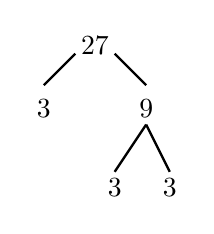
\begin{tikzpicture}
	\node at (-0.15,0) {$27$};
	\draw[line width=0.03cm] (-0.4,-0.1) -- (-0.8,-0.5);
	\node at (-0.8,-0.8) {$3$};
	\draw[line width=0.03cm]  (0.1,-0.1) -- (0.5,-0.5);
	\node at (0.5,-0.8) {$9$};
	
	\draw[line width=0.03cm] (0.5,-1) -- (0.1,-1.6);
	\node at (0.1,-1.8) {$3$};
	\draw[line width=0.03cm] (0.5,-1) -- (0.8,-1.6);
	\node at (0.8,-1.8) {$3$};
	\end{tikzpicture}
	\] \pspace

\item $185= 5 \cdot 37$
	\[
	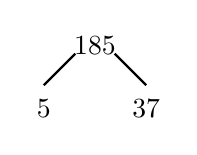
\begin{tikzpicture}
	\node at (-0.15,0) {$185$};
	\draw[line width=0.03cm] (-0.4,-0.1) -- (-0.8,-0.5);
	\node at (-0.8,-0.8) {$5$};
	\draw[line width=0.03cm]  (0.1,-0.1) -- (0.5,-0.5);
	\node at (0.5,-0.8) {$37$};
	\end{tikzpicture}
	\] 
\end{enumerate}



\newpage



% Problem 3
\problem{10} Compute each of the following by finding the divisors/multiples of the given integers:
        \begin{enumerate}[(a)]
        \item $\gcd(18, 24)$
        \item $\gcd(60, 125)$
        \item $\lcm(14, 20)$
        \item $\lcm(10, 21)$
        \end{enumerate} \pspace

\sol
\begin{enumerate}[(a)]
\item \phantom{.}\par
	\begin{table}[!ht]
	\centering
	\begin{tabular}{rl}
	18: & 1, 2, 3, \textbf{6}, 9, 18 \\
	24: & 1, 2, 3, 4, \textbf{6}, 8, 12, 24
	\end{tabular}
	\end{table} \par
Therefore, $\gcd(18, 24)= 6$. \pspace

\item \phantom{.}\par
	\begin{table}[!ht]
	\centering
	\begin{tabular}{rl}
	60: & 1, 2, 3, 4, \textbf{5}, 6, 10, 12, 15, 20, 30, 60 \\
	125: & 1, \textbf{5}, 25, 125
	\end{tabular}
	\end{table} \par
Therefore, $\gcd(60, 125)= 5$. \pspace

\item \phantom{.}\par
	\begin{table}[!ht]
	\centering
	\begin{tabular}{rl}
	14: & 14, 28, 42, 56, 70, 84, 98, 112, 126, \textbf{140} \\
	20: & 20, 40, 60, 80, 100, 120, \textbf{140}, 160, 180, 200
	\end{tabular}
	\end{table} \par
Therefore, $\lcm(14, 20)= 140$. \pspace

\item \phantom{.}\par
	\begin{table}[!ht]
	\centering
	\begin{tabular}{rl}
	10: & 10, 20, 30, 40, 50, 60, 70, 80, 90, 100, 110, 120, 130, 140, 150, \
160, 170, 180, 190, 200, \textbf{210} \\
	21: & 21, 42, 63, 84, 105, 126, 147, 168, 189, \textbf{210}
	\end{tabular}
	\end{table} \par
Therefore, $\lcm(10, 21)= 210$. \pspace
\end{enumerate}



\newpage



% Problem 4
\problem{10} Use the prime factorizations of the given integers to compute each of the following:
        \begin{enumerate}[(a)]
        \item $\gcd(142, 200)$
        \item $\lcm(72, 204)$
        \item $\gcd(2^{11} \cdot 3^8 \cdot 7^2 \cdot 17^4, 2^5 \cdot 3^2 \cdot 5^6 \cdot 11^{30})$
        \item $\lcm(2^{11} \cdot 3^8 \cdot 7^2 \cdot 17^4, 2^5 \cdot 3^2 \cdot 5^6 \cdot 11^{30})$
        \end{enumerate} \pspace

\sol
\begin{enumerate}[(a)]
\item 
	\[
	\gcd(142, 200)= \gcd(2 \cdot 71, 2^3 \cdot 5^2)= 2
	\] \pspace

\item 
	\[
	\lcm(72, 204)= \lcm(2^3 \cdot 3^2, 2^2 \cdot 3 \cdot 17)= 2^3 \cdot 3^2 \cdot 17= 1224
	\] \pspace

\item 
	\[
	\gcd(2^{11} \cdot 3^8 \cdot 7^2 \cdot 17^4, 2^5 \cdot 3^2 \cdot 5^6 \cdot 11^{30})= 2^5 \cdot 3^2= 288
	\] \pspace

\item 
	\[
	\begin{aligned}
	\lcm(2^{11} \cdot 3^8 \cdot 7^2 \cdot 17^4, 2^5 \cdot 3^2 \cdot 5^6 \cdot 11^{30})&= 2^{11} \cdot 3^8 \cdot 5^6 \cdot 7^2 \cdot 11^{30} \cdot 17^4 \\
	&= 14993131026926250123829433260382033579359008000000
	\end{aligned}
	\] 
\end{enumerate}



\newpage



% Problem 5
\problem{10} For each of the following, either convert the rational number from an improper fraction to a proper fraction or vice versa:
	\begin{enumerate}[(a)]
	\item $5\frac{6}{7}$
	\item $\frac{35}{3}$
	\item $-9\frac{3}{4}$
	\item $-\frac{26}{5}$
	\end{enumerate} \pspace

\sol
\begin{enumerate}[(a)]
\item 
	\[
	5 \tfrac{6}{7}= 5 + \dfrac{6}{7}= \dfrac{35}{7} + \dfrac{6}{7}= \dfrac{41}{7}
	\] \pspace

\item 
	\[
	\longdivision{35}{3}
	\] 
Then we have $35 - 3(11)= 35 - 33= 2$ so that $\dfrac{35}{3}= 11 \tfrac{2}{3}$. \pspace

\item 
	\[
	-9 \tfrac{3}{4}= -\left( 9 + \dfrac{3}{4} \right)= -\left( \dfrac{36}{4} + \dfrac{3}{4} \right)= -\dfrac{39}{4}
	\] \pspace

\item 
	\[
	\longdivision{26}{5}
	\] 
Then we have $26 - 5(5)= 26 - 25= 1$ so that $-\dfrac{26}{5}= -5 \tfrac{1}{5}$.
\end{enumerate}



\newpage



% Problem 6
\problem{10} Completely reduce the following rational numbers, showing all your work:
	\begin{enumerate}[(a)]
	\item $\dfrac{15}{33}$
	\item $-\dfrac{140}{90}$
	\item $\dfrac{210}{308}$
	\item $\dfrac{10}{21}$
	\end{enumerate} \pspace

\sol
\begin{enumerate}[(a)]
\item 
	\[
	\dfrac{15}{33}= \dfrac{\cancel{3} \cdot 5}{\cancel{3} \cdot 11}= \dfrac{5}{11}
	\] \pspace

\item 
	\[
	-\dfrac{140}{90}= -\dfrac{14 \cdot \cancel{10}}{9 \cdot \cancel{10}}= -\dfrac{14}{9}
	\] \pspace

\item 
	\[
	\dfrac{210}{308}= \dfrac{21 \cdot 10}{4 \cdot 77}= \dfrac{3 \cdot \cancel{7} \cdot 10}{4 \cdot \cancel{7} \cdot 11}= \dfrac{3 \cdot \cancel{10}^5}{\cancel{4}^2 \cdot 11}= \dfrac{3 \cdot 5}{2 \cdot 11}= \dfrac{15}{22}
	\] \pspace

\item 
	\[
	\dfrac{10}{21}= \dfrac{2 \cdot 5}{3 \cdot 7}= \dfrac{10}{21}
	\] 
\end{enumerate}



\newpage



% Problem 7
\problem{10} Simplifying as much as possible and showing all your work, compute the following:
	\begin{enumerate}[(a)]
	\item $\dfrac{12}{15} - \dfrac{5}{9}$
	\item $\dfrac{1}{6} + \dfrac{7}{12}$
	\item $-\dfrac{5}{12} + \dfrac{7}{18}$
	\item $2 + \dfrac{1}{3} - \dfrac{5}{2}$
	\end{enumerate} \pspace

\sol
\begin{enumerate}[(a)]
\item 
	\[
	\dfrac{12}{15} - \dfrac{5}{9}= \dfrac{36}{45} - \dfrac{25}{45}= \dfrac{36 - 25}{45}= \dfrac{11}{45}
	\] \pspace

\item 
	\[
	\dfrac{1}{6} + \dfrac{7}{12}= \dfrac{2}{12} + \dfrac{7}{12}= \dfrac{2 + 7}{12}= \dfrac{9}{12}= \dfrac{3}{4}
	\] \pspace

\item 
	\[
	-\dfrac{5}{12} + \dfrac{7}{18}= -\dfrac{15}{36} + \dfrac{14}{36}= \dfrac{-15 + 14}{36}= -\dfrac{1}{36}
	\] \pspace

\item 
	\[
	2 + \dfrac{1}{3} - \dfrac{5}{2}= \dfrac{12}{6} + \dfrac{2}{6} - \dfrac{15}{6}= \dfrac{12 + 2 - 15}{6}= -\dfrac{1}{6}
	\]
\end{enumerate} 



\newpage



% Problem 8
\problem{10} Simplifying as much as possible and showing all your work, compute the following:
	\begin{enumerate}[(a)]
	\item $\dfrac{15}{14} \cdot \dfrac{7}{33}$
	\item $\dfrac{\;\;\dfrac{5}{6}\;\;}{\dfrac{7}{15}}$
	\item $\dfrac{19}{4} \cdot -\dfrac{10}{9}$
	\item $\dfrac{\;\;\dfrac{2}{45}\;\;}{\dfrac{20}{21}}$
	\end{enumerate} \pspace

\sol
\begin{enumerate}[(a)]
\item 
	\[
	\dfrac{15}{14} \cdot \dfrac{7}{33}= \dfrac{\cancel{3} \cdot 5}{2 \cdot \cancel{7}} \cdot \dfrac{\cancel{7}}{\cancel{3} \cdot 11}= \dfrac{5}{22}
	\] \pspace

\item 
	\[
	\dfrac{\;\;\dfrac{5}{6}\;\;}{\dfrac{7}{15}}= \dfrac{5}{6} \cdot \dfrac{15}{7}= \dfrac{5}{\cancel{6}^2} \cdot \dfrac{\cancel{15}^5}{7}= \dfrac{25}{14}
	\] \pspace

\item 
	\[
	\dfrac{19}{4} \cdot -\dfrac{10}{9}= \dfrac{19}{\cancel{4}^2} \cdot -\dfrac{\cancel{10}^5}{9}= -\dfrac{95}{18}
	\] \pspace

\item 
	\[
	\dfrac{\;\;\dfrac{2}{45}\;\;}{\dfrac{20}{21}}= \dfrac{2}{45} \cdot \dfrac{21}{20}= \dfrac{\cancel{2}}{\cancel{3} \cdot 3 \cdot 5} \cdot \dfrac{\cancel{3} \cdot 7}{\cancel{2} \cdot 2 \cdot 5}= \dfrac{7}{150}
	\]
\end{enumerate} 



\newpage



% Problem 9
\problem{10} Showing all your work, convert the following rational numbers to decimals:
	\begin{enumerate}[(a)]
	\item $\dfrac{4}{9}$
	\item $\dfrac{7}{20}$
	\item $\dfrac{2}{11}$
	\end{enumerate} \pspace

\sol
\begin{enumerate}[(a)]
\item 
	\[
	\longdivision{4}{9}
	\] \pspace

\item 
	\[
	\longdivision{7}{20}
	\] \pspace

\item 
	\[
	\longdivision{2}{11}
	\] 
\end{enumerate}



\newpage



% Problem 10
\problem{10} Showing all your work, convert the following decimals to rational numbers:
	\begin{enumerate}[(a)]
	\item $0.7$
	\item $0.125$
	\item $0.121212\overline{12}$
	\end{enumerate} \pspace

\sol
\begin{enumerate}[(a)]
\item 
	\[
	0.7= \dfrac{7}{10}
	\] \pspace

\item 
	\[
	0.125= \dfrac{125}{1000}= \dfrac{3}{40}
	\] \pspace

\item \phantom{.}\par
	\begin{table}[!ht]
	\centering\small
	\begin{tabular}{rccc}
	& $100N$ & $=$ & $12.12121212\overline{12}$ \\ 
	$-$ & $N$ & $=$ & $\phantom{2}0.12121212\overline{12}$ \\ \hline
	& $99N$ & $=$ & $12$ \\[0.1cm]
	& $N$ & $=$ & $\frac{12}{99}$ \\[0.1cm]
	& $N$ & $=$ & $\frac{4}{33}$
	\end{tabular}
	\end{table} \par

	\[
	0.\overline{12}= \dfrac{4}{33}
	\] 
\end{enumerate}


\end{document}